\section{Parallel Implementations on CPU and GPU}
\frame{\tableofcontents[currentsection]}

\frame{ \frametitle{Introduction}
\begin{itemize}
\item Algorithmic improvement to $\ell_1$ minimization provided significant speed boost, but still not enough.
\item This section presents parallelized implementations of the face pipeline
\item There is ample parallelism available in the pipeline
\item Leverage the high levels of concurrency available in multi-core CPU and GPU architectures.
\end{itemize}
}

\frame{ \frametitle{CPU Hardware Overview}
\begin{itemize}
\item Large ammounts of cache (on-chip memory) compared to GPU
\item High clock speeds compared to GPU
\end{itemize}
}

\frame{ \frametitle{CPU Hardware Overview}
\begin{itemize}
\item Intel E5530, Dual-socket, quad-core Xeon
\item Each core has a private 32\,KiB L1 data cache 
\item Each core has a private 256\,KiB L2 cache.
\item Each chip has a shared 8\,MiB L3 cache.
\end{itemize}
}

\frame{ \frametitle{CPU Hardware Overview}
\begin{itemize}
\item Each of the 8 cores has a vector processor unit (SSE) that
can perform 4 single precision floating point operations concurrently.
\item Two levels of concurrency: {\em core-level} and {\em SSE-level}
\end{itemize}
}

\frame{ \frametitle{GPU Hardware Overview}
\begin{itemize}
\item High memory bandwidth compared to CPU
\item Much higher degree of concurrency compared to CPU
\end{itemize}
}
 
\frame{ \frametitle{GPU Hardware Overview}
\begin{itemize}
\item Single GTX480 GPU chip on PCIe expansion card
%\item Nvidia GTX480 programmed in C for CUDA
\item 15 {\em streaming multiprocessors} (SMs).
\item Each SM can execute 64 (two warps of 32 threads) floating point
operations concurrently.
\item Two levels of concurrency: {\em SM-level} and {\em thread-level} 
\end{itemize}
}

\frame{ \frametitle{GPU Hardware Overview}
\begin{itemize}
\item Each SM has 64 KiB of private L1 cache
\item The chip has 768 KiB of shared L2 cache
\end{itemize}
}

\newcommand{\tempscale}[0]{0.7}
\frame{ \frametitle{CPU and GPU cache comparison}
\centering
The larger algorithm data structures: \\
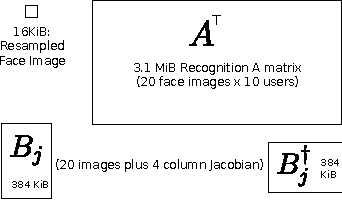
\includegraphics[scale=\tempscale]{../figures_ijcb/arrays.pdf} \\
The caches on a E5530 CPU: \\
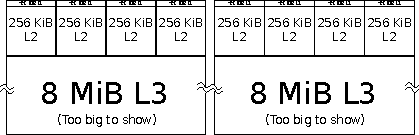
\includegraphics[scale=\tempscale]{../figures_ijcb/cpu_caches.pdf} \\
The caches on a GTX480 GPU: \\
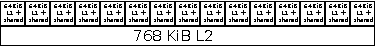
\includegraphics[scale=\tempscale]{../figures_ijcb/gpu_caches.pdf} \\
}

%\frame{ \frametitle{Limitations of CUDA programming model}
%}

\frame{ \frametitle{Face Recognition via ALM}
%\begin{algorithm}[t]
%\caption{\bf (Face Recognition via ALM)} \label{alg:alm_rec} 
\begin{algorithmic}[1]
\begin{small}
\STATE {\bf Input:} $\bb \in \Re^m$, $A \in \Re^{m \times n}$,
$\x_1 = \mathbf{0}$, $\e_1 = \bb$, $\y_1 =
\mathbf{0}$.
\WHILE{not converged ($k = 1,2,\ldots$)}
\STATE $\e_{k+1} = \shrink(\bb - A\x_k +
\frac{1}{\mu}\y_k, \frac{1}{\mu})$;
\STATE $t_1\leftarrow 1$, $\z_1 \leftarrow \x_k$, $\w_1 \leftarrow \x_k$;
\WHILE{not converged ($l = 1,2,\ldots$)}
\STATE $\w_{l+1} \leftarrow \shrink(\z_l +
\frac{1}{\gamma}A^T(\bb - A\z_l - \e_{k+1} +
\frac{1}{\mu}\y_k), \frac{1}{\mu\gamma})$;
\STATE $t_{l+1} \leftarrow \frac{1}{2}( 1 +
\sqrt{1+4t_l^2})$;
\STATE $\z_{l+1} \leftarrow \w_{l+1} + \frac{t_l - 1}{t_{l+1}}(\w_{l+1} - \w_l)$;
\ENDWHILE
\STATE $\x_{k+1} \leftarrow \w_{l}$,  \; $\y_{k+1} \leftarrow \y_k + \mu (\bb - A\x_{k+1} - \e_{k+1})$;
\ENDWHILE \STATE
{\bf Output:} $\x^* \leftarrow \x_k, \e^* \leftarrow \e_k$.
\end{small}
\end{algorithmic}
%\end{algorithm}
}

\frame{ \frametitle{Parallelization of SRC Recognition Stage}
\begin{itemize}
\item Single large $\ell_1$ minimization problem
\item Only one level of parallelism available: {\em pixel-level}
\item Essentially one essential parallelization strategy:\\
Map pixel-level parallelism onto both core-level and vector-level concurrency
\item Leverage built-in parallelization of MKL BLAS  and CUBLAS libraries
\item Array storage implicitly affects parallelization within the BLAS implementation
\end{itemize}
}
%\frame{ \frametitle{Parallelization of SRC Recognition Stage}
%\begin{itemize}
%\item Most operations map directly onto calls in the BLAS API.
%\item On the CPU, Intel's MKL BLAS can exploit both levels of concurrency on the CPU.
%\item On the GPU, Nvidia's CUBLAS exploits both levels of concurrency on the CPU.
%\item On the CPU, the remaining operations can be parallelized via manual threading (via OpenMP),
%and automatic vectorization (via the Intel ICC compiler).
%\item On the GPU, the remaining operations can be parallelized manually as CUDA kernels.
%\end{itemize}
%}


\frame{ \frametitle{Effect of Cache Size for solving a single minimization problem}
How does the speed of solving a single ALM problem at a time vary with problem size?
As a model for the recognition stage, consider solving the generic basis pursuit problem:
\begin{equation} 
\min \|\xx\|_1\quad \mbox{ subj. to }\quad \bb = A\xx
%\tag{\ref{eq:l1min}}
\end{equation}

Experiment Setup:
{\small
Random Gaussian $A \in \Re^{m \times 2*m}$, with normalized columns. 
Ground truth $\x_0$ also random Gaussian, 10\% sparsity, normalized to unit norm.
The measurement vector $\bb = A \x_0$.   
Termination when $\|\bx-\bx_0\| < \tau$ with $\tau=10^{-3}$.  
Running with single socket (4 cores, 8MB L3 cache).
}
}

\frame{ \frametitle{Effect of Cache Size for solving a single minimization problem}
%\frame{ \frametitle{Augmented Lagrangian Method (ALM) for general problem (wide A)}
\small
{\bf INPUT:} $\bb \in \Re^m$, $A=[A_1,\cdots, A_K] \in \Re^{m \times n}$, $\tau\leftarrow \max\mbox{eig}(A^TA)$, and constant $\rho>1$.
\begin{algorithmic}[1]
\WHILE{not converged ($k = 1,2,\ldots$)} 
\STATE $t_1 \leftarrow 1$, $\zz_1 \leftarrow \xx_k$, $\uu_1 \leftarrow \xx_k$ 
\WHILE{not converged ($l = 1,2,\ldots$)} 
\STATE $\uu_{l+1}  \leftarrow \shrink(\zz_l - \frac{1}{\tau}A^T(A\zz_l - \bb - \frac{1}{\mu_k}\blambda_k), \frac{1}{\mu_k\tau})$
\STATE $t_{l+1} \leftarrow \frac{1}{2}( 1 + \sqrt{1+4t_l^2})$
\STATE $\zz_{l+1} \leftarrow \uu_{l+1}+ \frac{t_l - 1}{t_{l+1}}(\uu_{l+1} - \uu_l)$ 
\ENDWHILE 
\STATE $\xx_{k+1} \leftarrow \uu_{l+1}$ 
\STATE $\blambda_{k+1} \leftarrow \blambda_k + \mu_k (\bb - A\xx_{k+1})$ 
\STATE $\mu_{k+1} \leftarrow \rho\cdot\mu_k$ 
\ENDWHILE 
\end{algorithmic}
{\bf OUTPUT:} $\xx^* \leftarrow \xx_k$.
}

\frame{ \frametitle{Effect of Cache Size for solving a single minimization problem}

\begin{center}
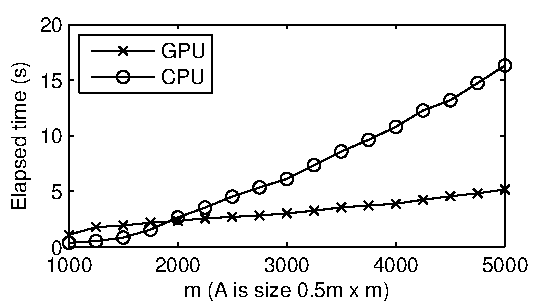
\includegraphics[width=3.5in]{../figures_ijcb/time_vs_matrix_size_constant_tol.pdf}
\end{center} 
%\caption{\small Comparison of $\ell_1$-minimization runtime vs. dimensions of $A$ on random data.} 
%\label{fig:random_data}

Crossover point occurs right where A reaches 8MB L3 cache size!
}

\frame{ \frametitle{Recognition stage runtime vs. face window resolution}
Benchmark ALM based Recognition stage running on real data:
Images of 10 users from Iterative Alignment Stage, running on Multi-PIE.
Vary image size: $32\times32$, $48 \times 48$, $64 \times 64$, $96 \times
96$, and $128 \times 128$.  
{
	\centering
	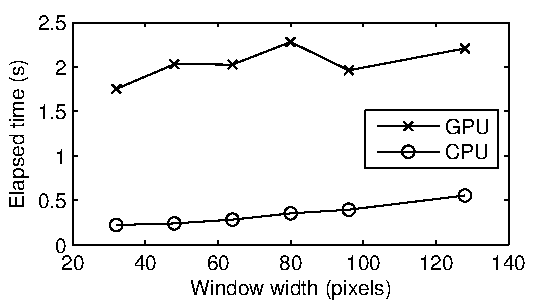
\includegraphics[width=2in]{../figures_ijcb/speedVsResolution.pdf} 
}

Problem size too small to run efficiently on GPU.

Runtime for both implementations low compared to alignment stage.
}

\frame{ \frametitle{Face Alignment via ALM}
\small
{\bf Input:} $\bb$, $A_i$, $\x_0 = \mathbf{0}$, $\tau_0$, and $J_0$.
\begin{algorithmic}[1]
\WHILE{not converged ($j = 1,2,\ldots$)}
\STATE Update $\bb_j \leftarrow \frac{\bb\circ \tau_{j-1}}{\|\bb\circ \tau_{j-1}\|}$; 
$B_j= [A_i, -J_{j-1}]$ and corresponding $(B_j^\dagger)^T$
%\STATE Initialize $\ww_0 = \mathbf 0$, $\blambda_0 = \mathbf 0$
\WHILE{not converged ($k = 1,2,\ldots$)}
\STATE $\uu_0\leftarrow \ww_{k-1}$; $\zz_0\leftarrow \e_{k-1}$
\WHILE{not converged ($l = 1,2,\ldots$)}
\STATE $\zz_l \leftarrow \shrink\left(\bb_j - B_j\uu_{l-1} + \frac{\blambda_{k}}{\mu_{k-1}}, \frac{1}{\mu_{k-1}}\right)$
\STATE $\uu_l \leftarrow B_j^\dagger \left(\bb_j - \zz_{l} + \frac{\blambda_{k-1}}{\mu_{k-1}} \right) $
\ENDWHILE
\STATE $\ww_k \leftarrow \uu_l$; $\e_k \leftarrow \zz_l$
\STATE $\blambda_{k} \leftarrow \blambda_{k-1} + \mu_{k-1} (\bb_j - B_j\ww_{k} - \e_{k})$
\STATE $\mu_{k} \leftarrow \rho\mu_{k-1}$
\ENDWHILE
\STATE Update $\e_j$, $\tau_j$, and $J_j$
\ENDWHILE
\end{algorithmic}
{\bf Output:} $\tau_i^*\leftarrow \tau_j, \e_i^*\leftarrow \e_j$
}

\frame{ \frametitle{Parallelism in the alignment stage}
\begin{itemize}
\item Many relatively small $\ell_1$ minimization problems that are solved repeatedly
\item Two levels of parallelism available: \emph{problem-level} and \emph{pixel-level}
\item $\ell_1$ minimization is interleaved with image rewarping.
\end{itemize}
}

\frame{ \frametitle{Parallelization of Iterative Alignment}
We consider two parallelizations of iterative alignment:
\begin{enumerate}
\item Alignment problems solved sequentially \\
\begin{itemize} 
\item problem-level parallelism unused
\item pixel-level parallelism mapped onto both vector-level and core-level hardware concurrency
\end{itemize}
\item Alignment problems solved concurrently \\
\begin{itemize} 
\item problem-level parallelism mapped onto core-level concurrency
\item pixel-level parallelism mapped onto vector-level concurrency
\end{itemize}
\end{enumerate}
}

\frame{ \frametitle{Benchmark of the Alignment Stage}
Experiment Setup: \\
CMU Multi-PIE Face Database.  \\
Gallery: Frontal images from session 1, 20 images per subject.\\
Test set: Frontal images from session 2 \\
Alignment is performed using a $64 \times 64$ window, similarity transformations,
manual initialization. \\
The number of gallery subjects is varied.
}

\frame{ \frametitle{Alignment stage runtime vs. size of training database.}
\centering
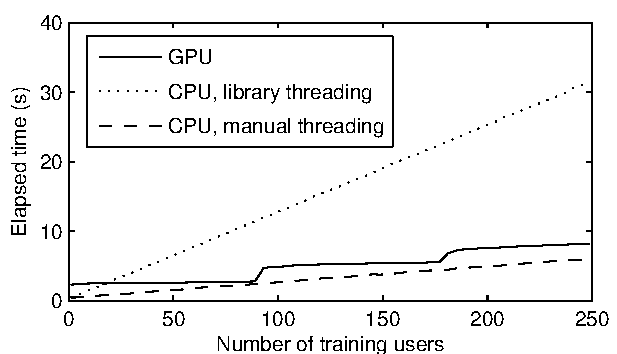
\includegraphics[width=3in]{../figures_ijcb/alignment_runtime_graph.pdf}
}


%\item Most operations map directly onto calls in the BLAS API.
%\item On the CPU, Intel's MKL BLAS can exploit both levels of concurrency on the CPU.
%\item On the GPU, Nvidia's CUBLAS exploits both levels of concurrency on the CPU.
%\item On the CPU, the remaining operations can be parallelized via manual threading (via OpenMP),
%and automatic vectorization (via the Intel ICC compiler).
%\item On the GPU, the remaining operations can be parallelized manually as CUDA kernels.
%\end{itemize}
%}

%%\subsection{Recap}
\frame{ \frametitle{Existing Architectures are already fast} CPU and GPU architectures competitive, and
both benefit dramatically from proper parallelization.  Implementation on GPU much more painful; no SM level
libraries}
\frame{ \frametitle{Improving hardware architectures} CPU/GPU hybrids: Intel Knight's Corner and AMD's APU}

